\chapter{Algoritmy řešící [n,k]-Mastermind}

\section{Kategorie algoritmů}
% přidat definici algoritmu, který řeší mastermind - vytvoří posloupnost kódů, která končí tajným kódem s nejlepším ohodnocením. 
Algoritmy řešící hru Mastermind lze rozdělit do dvou kategorií, \textbf{deterministické} a \textbf{nedeterministické}. Deterministický algoritmus pro dva shodné stavy volí další krok vždy jednoznačně. Nemůže se tedy stát, že by deterministický algoritmus pro dva stejné vstupy vrátil odlišné výsledky. Nedeterministické algoritmy naproti tomu mohou mít v každém stavu na výběr z více následujících kroků. Volit mohou například podle nějakého pravděpodobnostního rozdělení. Není tedy zaručeno, že pro stejný vstup vrátí vždy identický výsledek.

Deterministické algoritmy řešící hru Mastermind mohou mít velikou časovou složitost. To se snaží řešit nedeterministické algoritmy, které hledají rovnováhu mezi časovou složitostí a dobrými výsledky. 
% Hlavní předností deterministických algoritmů je záruka výsledku. Na druhou stranu ale tyto typy algoritmů mohou mít velikou časovou složitost, protože jsou často založeny na procházení všech možností pokračování. To se snaží řešit nedeterministické algoritmy, které hledají rovnováhu mezi časovou složitostí a dobrými výsledky. 
V této práci budeme zkoumat pouze deterministické algoritmy. 

% šlo by zmínit výhody a nevýhody (ne)deterministických algoritmů
% Popsat algoritmy, které hrají pouze kandidáty????


\section{Deterministické algoritmy}
% mozna napsat pozdeji ... Všechny deterministické algoritmy, které budeme srovnávat ...

\subsubsection{Stav hry}
V každém kroku algoritmů vycházíme z určitého stavu hry, pro který daná metoda vybírá další pokus. Stav je posloupnost pokusů s ohodnocením a jsou to přesně ty informace, které má hráč [n,k]-Mastermindu k dispozici, a na základě kterých volí následující tah.

\begin{definice}[Stav]\label{stav}
   Nechť $j \in \mathbb{N}$, $u_1, \dots , u_j$ jsou kódy a $r_i = (b_i,w_i), i \in \{1,2,\dots,j\}$ ohodnocení. Stav definujeme jako posloupnost $((u_1, r_1), \dots, (u_m, r_m))$. Počáteční stav definujeme jako prázdnou posloupnost $()$.
\end{definice}

% Vazby stavů budeme interpretovat jako v kořenovém stromu, kde vrcholy odpovídají stavům. Hrany znázorňují pokusy s ohodnocením, které [n,k]-Mastermind posouvají do dalších stavů. 
Stavy hry a vazby mezi nimi popíšeme grafem. Hrany znázorňují pokusy s ohodnocením, které hru [n,k]-Mastermind posouvají do dalších stavů. 
\begin{definice}[Strom \text{[n,k]-Mastermindu}]
  Strom \text{[n,k]-Mastermindu} definujeme jako kořenový strom na množině stavů. Kořenem je počáteční stav. Ze stavu $A = \left((u_1, r_1), (u_2,r_2), \dots, (u_j,r_j)\right)$ do stavu $B = \left((w_1, s_1), (w_2,s_2), \dots, (w_l,s_l)\right)$ vede hrana právě tehdy, když $l = j+1$ a $\forall i \in \{1,2,\dots, j\} \colon (u_i, r_i) = (w_i, s_i)$. Tuto hranu značíme dvojicí $w_l, s_l$. 
\end{definice}

Obrázek \ref{fig22prvnitah} zobrazuje počáteční stav [2,2]-Mastermindu a všechny stavy, do kterých se lze dostat po prvním pokusu. 


\begin{figure}[h!]
    \centering
    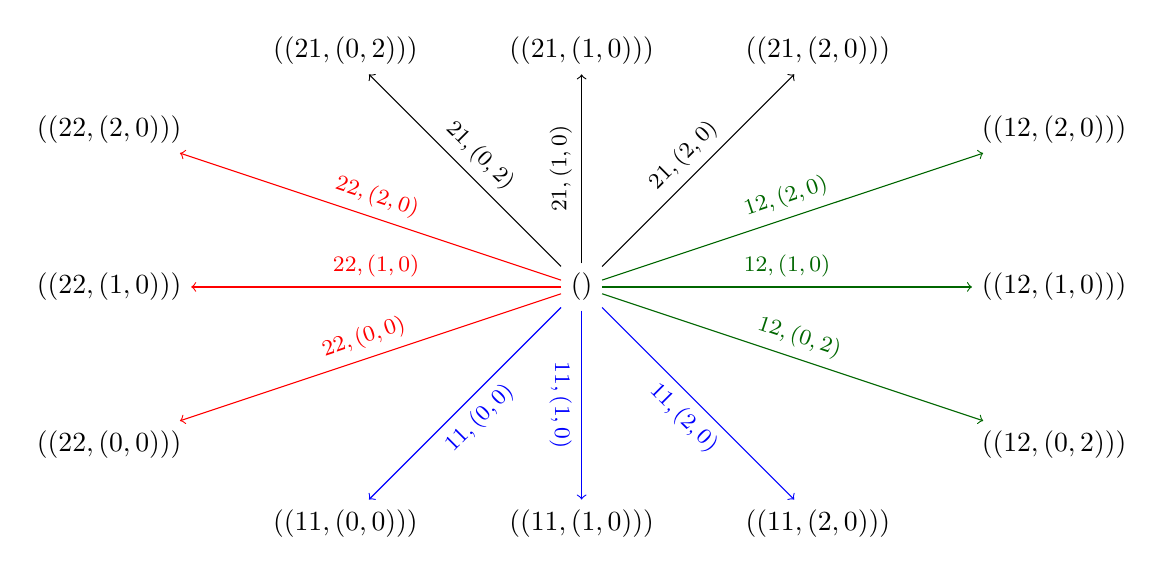
\begin{tikzpicture}
    \node (1) at (0,0) {$()$};
    
    \node (2) at (-3,-3) {$((11,(0,0)))$};
    \draw[->,blue] (1) -- (2) node[pos=0.5, below, sloped] {\footnotesize$11,(0,0)$};
    \node (3) at (0,-3) {$((11,(1,0)))$};
    \draw[->,blue] (1) -- (3) node[pos=0.5, below, sloped] {\footnotesize$11,(1,0)$};
    \node (4) at (3,-3) {$((11,(2,0)))$};
    \draw[->,blue] (1) -- (4) node[pos=0.5, below, sloped] {\footnotesize$11,(2,0)$};
    
    \node (5) at (6,-2) {$((12,(0,2)))$};
    \draw[->,black!60!green] (1) -- (5) node[pos=0.5, above, sloped] {\footnotesize$12,(0,2)$};
    \node (6) at (6,0) {$((12,(1,0)))$};
    \draw[->,black!60!green] (1) -- (6) node[pos=0.5, above, sloped] {\footnotesize$12,(1,0)$};
    \node (7) at (6,2) {$((12,(2,0)))$};
    \draw[->,black!60!green] (1) -- (7) node[pos=0.5, above, sloped] {\footnotesize$12,(2,0)$};

    \node (8) at (-3,3) {$((21,(0,2)))$};
    \draw[->] (1) -- (8) node[pos=0.5, above, sloped] {\footnotesize$21,(0,2)$};
    \node (9) at (0,3) {$((21,(1,0)))$};
    \draw[->] (1) -- (9) node[pos=0.5, above, sloped] {\footnotesize$21,(1,0)$};
    \node (10) at (3,3) {$((21,(2,0)))$};
    \draw[->] (1) -- (10) node[pos=0.5, above, sloped] {\footnotesize$21,(2,0)$};

    \node (11) at (-6,-2) {$((22,(0,0)))$};
    \draw[->,red] (1) -- (11) node[pos=0.5, above, sloped] {\footnotesize$22,(0,0)$};
    \node (12) at (-6,0) {$((22,(1,0)))$};
    \draw[->,red] (1) -- (12) node[pos=0.5, above, sloped] {\footnotesize$22,(1,0)$};
    \node (13) at (-6,2) {$((22,(2,0)))$};
    \draw[->,red] (1) -- (13) node[pos=0.5, above, sloped] {\footnotesize$22,(2,0)$};


    \end{tikzpicture}
    \caption{Graf všech následníků počátečního stavu [2,2]-Mastermindu}
    \label{fig22prvnitah}
\end{figure}

Stavy, do kterých ze stavu $A$ vede nějaká hrana nazýváme následníky stavu $A$. 
%Zavádíme definici potomka množiny, která s potomkem stavu přímo souvisí. 

\begin{definice}[Následník stavu]\label{potomek}
  % Uvažujme [n,k]-Mastermind s nějakým tajným kódem $v\in H_{n,k}$. 
  % Nechť $S$ je množina všech ohodnocení v $H_{n,k}$. Nechť $A = \left((u_1, r_1), \dots, (u_j,r_j)\right)$ je stav, $u \in H_{n,k}$ je kód a $r \in S$ ohodnocení. Potomka stavu $A$ vzhledem ke kódu $u$ a ohodnocení $r$ definujeme jako stav $A_{u,r} = (\left((u_1, r_1), \dots, (u_j,r_j) ,(u,r)\right)$. 
  
  Následník stavu $A$ vzhledem ke kódu $u$ a ohodnocení $r$ je stav, do kterého vede ze stavu $A$ hrana $(u,r)$ a značíme ho $A_{u,r}$. 
  
  %Nechť $K \subset H_{n,k}$ je množina kódů, potom potomka množiny $K$ vzhledem ke kódu $u$ a ohodnocení $r$ definujeme jako množinu
  %\[K_{u,r} = \{w \in K \mid s(u,w) = r\}.\] 
\end{definice}

Průběh [n,k]-Mastermindu s nějakým tajným kódem $v$ lze sledovat ve stromu [n,k]-Mastermindu. Nechť $A$ je stav a hráč zvolí další pokus $u$. Touto volbou hráč vybral část následníků, do kterých se stav hry může dostat. Jsou to právě následníci stavu $A$ vzhledem ke kódu $u$. Zadavatel ohodnotí kód $u$ vzhledem ke kódu $v$ ohodnocením $r$. Ohodnocením určí, který stav z následníků $A$ vzhledem ke kódu $u$ bude následovat. Hráč tedy může vybrat jako následující pokus ten, který bude mít nejvhodnější vrstvu následníků stavu $A$ (například podle množin kandidátů definovaných níže). Z těchto následníků ale neví, do kterého se hra dostane, protože nezná ohodnocení s tajným kódem. 


\subsubsection{Kandidát}
Pro každý stav lze nalézt množinu kódů, které by podle dostupných informací mohly být tajným kódem. 
% Jde o ty kódy, které mají s kódy ve stavu stejné ohodnocení jako příslušná ohodnocení ve stavu. 

\begin{definice}[Množina kandidátů]\label{kandidat}
  Pro počáteční stav definujeme množinu kandidátů jako celý prostor kódů $H_{n,k}$. Nechť $A = \left((u_1, r_1), (u_2,r_2), \dots, (u_j,r_j)\right), u_i \in H_{n,k}, r_i \in \N _0 \times \N _0$ je stav. Množinu kandidátů stavu $A$ definujeme jako
  \[K = \{w \in H_{n,k} \mid s(u_i,w) = r_i,  i \in \{1,2,\dots ,j\} \}.\]
  Kód z této množiny nazveme kandidát stavu $A$. 
  
  %Řekneme, že kód $u \in H_{n,k}$ je kandidát stavu $A$, pokud $s(u,u_i) = r_i \hspace{5px} \forall i \in \{1, \dots j\}$. 

  % Dále definujeme funkci $J$, která stavu přiřadí jeho množinu kandidátů.
  % \begin{align*}
  %     J \colon (H_{n,k} \times S)^+ &\to \mathbb{R} \\
  %       \left((u_1, r_1), (u_2,r_2), \dots, (u_j,r_j)\right) &\mapsto \{u \in H_{n,k} \mid s(u,u_i) = r_i \hspace{5px} \forall i \in \{1, \dots j\} \} 
  % \end{align*}
\end{definice}
Velikost a struktura množiny kandidátů určuje, jak blízko jsme uhodnutí tajného kódu.

% Množina kandidátů dává intuici za tím, jak blízko jsme uhádnutí tajného kódu. V případě, že množina kandidátů je jednoprvková, tak nám je znám tajný kód. Pokud je množina kandidátů veliká, nejspíš ještě budeme k rozlišení tajného kódu potřebovat více pokusů.


\begin{definice}[Potomek množiny]\label{lemmasjednocenipotomku}
  % Uvažujme [n,k]-Mastermind s nějakým tajným kódem $v\in H_{n,k}$. 
  Nechť $S$ je množina všech ohodnocení v $H_{n,k}$. Nechť $K$ je podmnožina $H_{n,k}$, $ u \in H_{n,k}$ je kód a $r \in S$ ohodnocení. Potomka množiny $K$, vzhledem ke kódu $u$ a ohodnocení $r$ definujeme jako množinu 
  \[K_{u,r} = \{w \in K \mid s(u,w) = r\}.\] 
\end{definice}

Z definice plyne, že $\bigcup_{r\in S} K_{u,r} \subset K$. Zároveň žádný kód $w \in K$ nemůže mít s kódem $u$ dvě různá ohodnocení, a tedy sjednocení je disjunktní. Navíc pro každý kód $w \in K$ platí, že $w \in K_{u, s(u,w)}$ a tedy platí následující lemma.

\begin{lemma}[Vztah množiny s jejími potomky]
    Nechť $S$ je množina všech ohodnocení kódů v $H_{n,k}$. Pro každou množinu $K \subset H_{n,k}$ a kód $u \in H_{n,k}$ platí
    \[K = \bigsqcup_{r\in S} K_{u,r}\]
\end{lemma}


% \begin{dukaz}
%     Dokážeme obě inkluze. Z definice $K_{u,r}$ platí 
%     \[\bigsqcup_{r\in S} K_{u,r} \subset K.\] 
%     Nechť $u \in H_{n,k}$. Potom pro každý kód $w \in K$ platí, že $w \in K_{u, s(u,w)}$ a tedy 
%     \[K \subset \bigsqcup_{r\in S} K_{u,r}.\] 
%     Zároveň žádný kód $w \in K$ nemůže mít s kódem $u$ dvě různá ohodnocení, a tedy sjednocení je disjunktní. 
% \end{dukaz}

% \begin{definice}[Graf \text{[n,k]-Mastermindu}]
%   Uvažujeme množinu vrcholů $\mathcal{V} = \mathcal{P}(H_{n,k})$ a množinu orientovaných hran $\mathcal{E}$ mezi vrcholy a jejich potomky. 
%   Cestu definujeme jako posloupnost navazujících hran. 
%   Definujeme $V \subset \mathcal{V}$ jako množinu vrcholů, do kterých vede cesta z vrcholu $H_{n,k}$. Graf [n,k]-Mastermindu definujeme jako indukovaný podgraf grafu $(\mathcal{V}, \mathcal{E})$ množinou $V$. Hranu $(K, K_{u,r})$ budeme značit jako hranu $(u,r)$ z vrcholu $K$.
% \end{definice}
\begin{lemma}[Vztah následníků a potomků]\label{lemmapotomcistavuakandidati}
    Označíme-li $K$ množina kandidátů stavu $A = \left((u_1, r_1), (u_2,r_2), \dots, (u_j,r_j)\right)$, tak $K_{u,r}$ je množina kandidátů stavu $A_{u,r}$.
\end{lemma}
\begin{dukaz}
    $K_{u,r} = \{w \in K \mid s(u,w) = r\}$. Navíc $K = \{z \in H_{n,k} \mid s(u_i,z) = r_i,  i \in \{1,2,\dots ,j\} \}$. Lemma plyne z definice množiny kandidátů stavu $A_{u,r}$.
\end{dukaz}


\begin{definice}[Multigraf prostoru kódů]
  Uvažujeme multigraf $M_{n,k}$ na množině vrcholů $\mathcal{V} = \mathcal{P}(H_{n,k})$, kde z vrcholu $K_1$ do vrcholu $K_2$ vede hrana obarvená $(u,r)$, pokud $K_2$ je potomek $K_1$ vzhledem ke kódu $u$ a ohodnocení $r$.
\end{definice}

\begin{definice}[Orientovaná cesta]
    Orientovanou cestou (dále jen cestou) rozumíme prázdnou posloupnost, nebo posloupnost navazujících hran. 
    % Řekneme, že do vrcholu $K_2$ vede cesta z vrcholu $K_1$, pokud 
\end{definice}

\begin{definice}[Multigraf \text{[n,k]-Mastermindu}]
  Multigraf [n,k]-Mastermindu definujeme jako podgraf multigrafu $M_{n,k}$ množinou vrcholů, do kterých vede cesta z vrcholu $H_{n,k}$. Značíme ho $M_{n,k}^*$.
  
  %a množinu orientovaných hran $\mathcal{E}$ mezi vrcholy a jejich potomky. 
  %Cestu definujeme jako posloupnost navazujících hran. 
  %Definujeme $V \subset \mathcal{V}$ jako množinu vrcholů, do kterých vede cesta z vrcholu $H_{n,k}$. Graf [n,k]-Mastermindu definujeme jako indukovaný podgraf grafu $(\mathcal{V}, \mathcal{E})$ množinou $V$. Hranu $(K, K_{u,r})$ budeme značit jako hranu $(u,r)$ z vrcholu $K$.
\end{definice}

\begin{pozn}
    Cestu je posloupnost navazujících hran. Mezi dvěma vrcholy může vést více hran, jak je vidět na obrázku \ref{fig22prvnitahmnoziny}, který zobrazuje potomky $H_{2,2}$ vzhledem ke všem kódům a ohodnocením. 
\end{pozn}

\begin{figure}[h!]
    \centering
    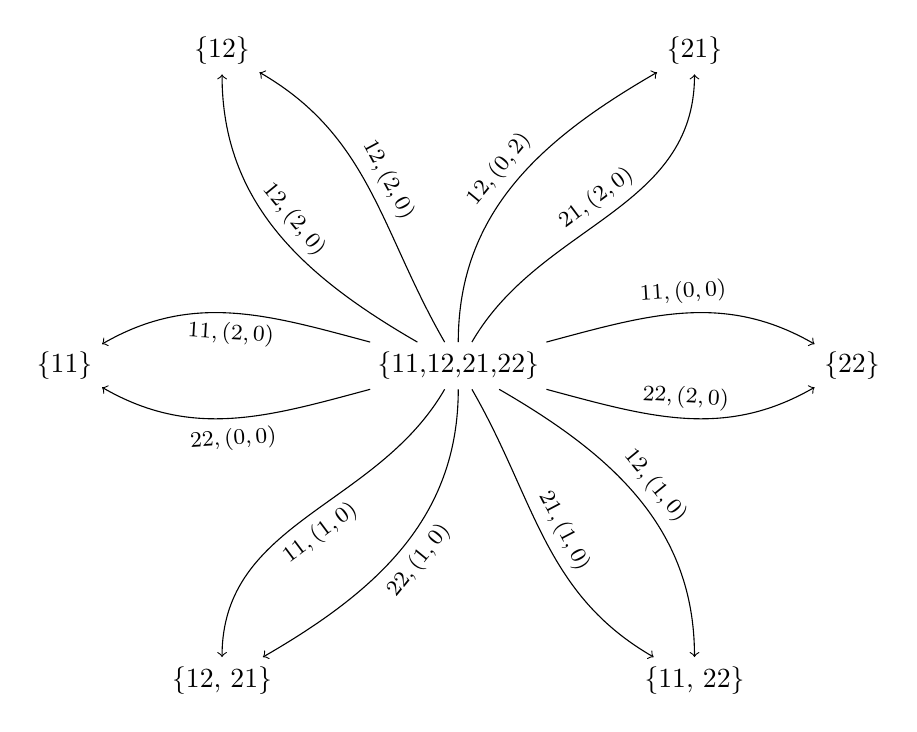
\begin{tikzpicture}
    \node (1) at (0,0) {\{11,12,21,22\}};
    \node (4) at (-5,0) {\{11\}};
    \draw[->] (1) to[out=165, in=30]  node[midway, below, sloped] {\footnotesize$11,(2,0)$} (4);
    \draw[->] (1) to[out=-165, in=-30] node[pos=0.5, below, sloped] {\footnotesize$22,(0,0)$} (4);
    \node (7) at (-3,4) {\{12\}};
    \draw[->] (1) to[out=150, in=-90] node[pos=0.5, above, sloped] {\footnotesize$12,(2,0)$} (7) ;
    \draw[->] (1) to[out=120, in=-30] node[pos=0.5, above, sloped] {\footnotesize$12,(2,0)$} (7);
    \node (5) at (3,4) {\{21\}};
    \draw[->] (1) to[out=90, in=-150] node[pos=0.5, above, sloped] {\footnotesize$12,(0,2)$} (5);
    \draw[->] (1) to[out=60, in=-90] node[pos=0.5, above, sloped] {\footnotesize$21,(2,0)$} (5);
    \node (2) at (5,0) {\{22\}};
    \draw[->] (1) to[out=15, in=150] node[midway, above, sloped] {\footnotesize$11,(0,0)$} (2);
    \draw[->] (1) to[out=-15, in=-150] node[midway, above, sloped] {\footnotesize$22,(2,0)$} (2);
    \node (6) at (3,-4) {\{11, 22\}};
    \draw[->] (1) to[out=-30, in=90] node[pos=0.5, above, sloped] {\footnotesize$12,(1,0)$} (6);
    \draw[->] (1) to[out=-60, in=150] node[pos=0.5, above, sloped] {\footnotesize$21,(1,0)$} (6);
    \node (3) at (-3,-4) {\{12, 21\}};
    \draw[->] (1) to[out=-120, in=90] node[midway, below, sloped] {\footnotesize$11,(1,0)$} (3);
    \draw[->] (1) to[out=-90, in=30] node[midway, below, sloped] {\footnotesize$22,(1,0)$} (3);
    \end{tikzpicture}
    \caption{Multigraf všech potomků $H_{2,2}$}
    \label{fig22prvnitahmnoziny}
\end{figure}

% zdroj - wikipedie, https://en.wikipedia.org/wiki/Directed_acyclic_graph
\begin{definice}[Orientovaný acyklický multigraf]
    Řekneme, že orientovaný multigraf $H$ je orientovaný acyklický, pokud neexistuje cesta, která začíná i končí ve stejném vrcholu a není v tomto vrcholu konstantní.
\end{definice}

\begin{pozorovani}
    Multigraf [n,k]-Mastermindu je orientovaný acyklický multigraf. 
\end{pozorovani}
\begin{dukaz}
    Nechť $K_1$ a $K_2$ jsou vrcholy. Pokud z vrcholu $K_1$ vede cesta do vrcholu $K_2$, $K_2 \subseteq K_1$. Pokud $K_2 \neq K_1$, potom $K_2 \subset K_1$. Pokud existuje nějaká cesta z $K_1$ přes $K_2$ zpět do $K_1$, potom $K_2 \subset K_1 \subset K_2$, což je spor. Tedy neexistuje nekonstantní orientovaná cesta v [n,k]-Mastermindu a je to tedy orientovaný acyklický multigraf.
\end{dukaz}

% multigraf je "directed acyclic graph"
\begin{definice}[Rozvinutí orientovaného acyklického multigrafu]
    Nechť $H$ je orientovaný acyklický multigraf s jedním kořenem. 
    Potom definujeme jeho rozvinutí jako následný strom:
    Definujeme množinu vrcholů $V$ jako množinu cest v multigrafu $H$ začínající v kořeni. 
    Hrany definujeme podle následujícího předpisu. Nechť $A, B \in V$ jsou vrcholy. Potom z vrcholu $A \in V$ do vrcholu $B \in V$ vede hrana právě tehdy, když cesta $B$ vznikne z cesty $A$ prodloužením o jednu hranu. Tuto hranu obarvujeme poslední hranou cesty $B$. 
\end{definice}

\begin{veta}
    Strom [n,k]-Mastermindu je rozvinutím multigrafu [n,k]-Mastermindu.
\end{veta}

% Díky Lemmatu \ref{lemmapotomcistavuakandidati} můžeme popsat vztah mezi stromem a grafem [n,k]-Mastermindu. Nějaký vrchol $K$ grafu je množina kandidátů všech stavů, které odpovídají cestám z $H_{n,k}$ do tohoto vrcholu. 

% \begin{tvrz}[Vztah multigrafu a stromu \text{[n,k]-Mastermindu}]\label{tvrzenimultigrafastrom}
%     Nechť $A = \left((u_1, r_1), (u_2,r_2), \dots, (u_j,r_j)\right)$ je stav. a $K_1$ je jeho množina kandidátů. Nechť $K_2$ odpovídá vrcholu na konci cesty $A$ z $H_{n,k}$ multigrafem [n,k]-Mastermindu. Potom $K_1 = K_2$.  
% \end{tvrz}
% \begin{dukaz}
%     Postupujeme indukcí podle délky stavu. Nechť délka stavu je $1$, tvrzení platí díky lemmatu \ref{lemmapotomcistavuakandidati}. Nechť tvrzení platí pro $j\in \mathbb{N}, j\geq 2$. Potom $A = B_{u_{j+1}, r_{j+1}}$ pro nějaký stav $B$, kde množinu kandidátů $B$ označíme $K$. Potom $K$ je konec cesty $B$ z $H_{n,k}$ multigrafem [n,k]-Mastermindu z indukčního předpokladu. Potom z lemmatu \ref{lemmapotomcistavuakandidati} platí, že $K_{u_j, r_j}$, která je koncem cesty $A$ z $H_{n,k}$, je množina kandidátů stavu $A$. 
% \end{dukaz}


 





% \begin{pozn}
%     Všimněme si, že $K_{u,r} \subset K \hspace{3px}\forall u\in H_{n,k} \hspace{3px}\forall r\in S$. Navíc pro každou množinu $K \subset H_{n,k}$ a kód $u \in H_{n,k}$ platí
%     \[K = \bigsqcup_{r\in S} K_{u,r}\]
%     protože pro každý kód $w \in K$ platí, že $w \in K_{u, s(u,w)}$.
%     %, tedy že $w$ náleží do potomka $K$ vzhledem ke kódu $u$ a ohodnocení $s(u,w)$. 
% \end{pozn}
% \begin{definice}[Graf \text{[n,k]-Mastermindu}]
%   Uvažujeme množinu vrcholů $\mathcal{V} = \mathcal{P}(H_{n,k})$ a množinu orientovaných hran $\mathcal{E}$ mezi vrcholy a jejich potomky. Cestu definujeme jako posloupnost navazujících hran. Definujeme $V \subset \mathcal{V}$ jako množinu vrcholů, do kterých vede cesta z vrcholu $H_{n,k}$. Graf [n,k]-Mastermindu definujeme jako indukovaný podgraf grafu $(\mathcal{V}, \mathcal{E})$ množinou $V$. Hranu $(K, K_{u,r})$ budeme značit jako hranu $(u,r)$ z vrcholu $K$.
% \end{definice}




% ======================== napsat u obecneho algoritmu =====================


\subsubsection{Obecný algoritmus}
Nyní přistoupíme k popisu skupiny deterministických algoritmů řešící hru [n,k]-Mastermind. V této práci popisujeme algoritmy, které pro libovolný stav $A$ vybírají další pokus podle množiny kandidátů stavu $A$. 
Pro dva různé stavy, které ale mají shodnou množinu kandidátů je problém nalezení dalšího kódu ekvivalentní. Předpokládáme totiž, že všechny kódy mohou být tajným kódem se stejnou pravděpodobností. 
Tento výběr popíšeme pomocí dvou funkcí, valuace a strategie. 


% Algoritmy popisujeme podle funkcí, které pro jakýkoliv stav naleznou další pokus. Nazýváme je, valuace a strategie. 

% Tyto funkce definujeme pro množiny kandidátů stavů. 

% Množiny kandidátů pro nás budou sloužit jako vnitřní stavy, pomocí kterých vybíráme další pokusy. Pro dva různé stavy, které ale mají shodnou množinu kandidátů je problém nalezení dalšího kódu ekvivalentní. Předpokládáme totiž, že všechny kódy mohou být tajným kódem se stejnou pravděpodobností. 



% Pro zjednodušení tyto funkce definujeme pro množiny kandidátů stavů. Pro dva různé stavy, které ale mají shodnou množinu kandidátů je problém nalezení dalšího kódu ekvivalentní. Předpokládáme totiž, že všechny kódy mohou být tajným kódem se stejnou pravděpodobností. Stejné množiny kandidátů pro dva různé stavy lze například dosáhnout prohozením prvků stavu. 

% Ve chvíli, kdy mají nějaké dva stavy stejnou množinu kandidátů, nezáleží na tom, jaké prvky stav obsahuje. Platí, že při následném zvolení stejných pokusů pro oba stavy dosáhneme stejného výsledku. Dojdeme ke stejnému konečnéme stavu.

% Pro dva různé stavy, které ale mají shodnou množinu kandidátů je problém nalezení dalšího kódu ekvivalentní. Předpokládáme totiž, že všechny kódy mohou být tajným kódem se stejnou pravděpodobností. Stejné množiny kandidátů pro dva různé stavy lze například dosáhnout prohozením prvků stavu. 


% K popisu výběru dalšího tahu algoritmy nebudou používat stav hry jako v definici \ref{defstav}. Místo toho vybírají další kód za pomocí množiny kandidátů tohoto stavu. 

% Našim cílem je totiž co nejlépe rozlišit, který kandidát je tajným kódem. Různé stavy které ale mají stejnou množinu kandidátů se v této informaci neliší. Proto výběr dalšího tahu lze vztáhnout pouze na množinu kandidátů aktuálního stavu. 



% U této definice si nejsem jistý, jak to smyslupně definovat. Vazba "která lz e vyjádřit pomocí potomků" se mi moc nelíbí - definovat valuaci a až potom jednokrokové valuace
\begin{definice}[Valuace]
    Nechť $G = (V,E)$ je graf [n,k]-Mastermindu a $K \in V$ je vrchol. Potom valuaci vzhledem k množině $K$ definujeme jako funkci $f_K(u) \colon H_{n,k} \to \mathbb{R}$.
\end{definice}


Valuace bude v algoritmech sloužit pro vyčíslení vhodnosti kódu $u$ jako dalšího pokusu pro stav s množinou kandidátů $K\subset H_{n,k}$. Tato hodnota bude obvykle záviset na potomcích $K$ vzhledem ke kódu $u$. Potomci $K$ vzhledem ke kódu $u$ totiž určují množiny kandidátů možných následující stavů v případě, kdy zvolíme kód $u$ jako další pokus (Lemma \ref{lemmapotomcistavuakandidati}). Valuace nám umožňuje ohodnotit kód podle toho, jak dobré jsou jeho následující stavy. Valuace by nemusela být omezená na následující vrstvu. Mohla by odkazovat na stavy o více než jednu hranu dál.

\begin{prikl}\label{prjednokrokfce}
    Funkce $f_K$ je příklad valuace, která kódu $u$ přiřadí maximální počet kódů potomka $K$ vzhledem ke kódu $u$.
    % jednokrokov8 funkce je taková, která kódu $u$ přiřadí hodnotu, která lze vyjádřit pomocí potomků $K$ vzhledem ke kódu $u$.
    \begin{align*}
        f_K \colon H_{n,k} &\to \mathbb{R} \\
        u &\mapsto \max_{r\in S} |K_{u,r}|
    \end{align*}
    % Pro $K = H_{2,2}$ z obrázku \ref{fig22prvnitah} má $f_{K}$ konstantní hodnotu $\frac{3}{2}$.
\end{prikl}
% množinu kandidátů na tajný kód


\begin{definice}[Strategie]
    Nechť $\mathcal{F} = \{f_K\colon H_{n,k} \to \mathbb{R} \mid K \subset H_{n,k}\}$ je prostor valuací. Potom řekneme, že zobrazení $F \colon \mathcal{F} \to \mathbb{R}$ je strategie, pokud pro každou $f_K \in \mathcal{F}$ existuje $u\in H_{n,k}$ takové, že $F(f_K) = f_K(u)$.
\end{definice}
% Strategie určitým způsobem slouží k výběru následujícího kódu. 
%Zjednodušeně řečeno slouží k určení, 
Strategie určuje kritérium, podle kterého se vybírá další pokus v závislosti na valuaci. Budeme totiž vybírat právě ty kódy, které mají valuaci rovnou hodnotě strategie pro danou funkci. 

% v této práci bude určovat, zda chceme vybírat kódy s vyšší nebo nižší hodnotou valuace.
%Použití bude popsáno níže v popisu algoritmu \ref{alg-default}. 

\begin{prikl}\label{prstrategie}
    Funkce $F$ je strategie, která funkci $f_K \in \mathcal{F} = \{f_K\}$ přiřadí její maximální hodnotu na $H_{n,k}$.
    \[F(f_K) =  \max_{u\in H_{n,k}} f_K(u)\]
    Strategie je dobře definovaná, protože maximum na konečné množině reálných čísel má vždy jednoznačnou hodnotu a existuje $u\in H_{n,k}$, pro který platí $f_K(u) = \max_{u\in H_{n,k}} f_K(u)$.
\end{prikl}

\begin{definice}[Deterministický algoritmus]\label{defobecnyalg}
    Deterministický algoritmus s prostorem valuací $\mathcal{F}$ a strategií $F$ je definovaný podle předpisu funkce \textsc{Solve} v algoritmu \ref{alg-default} jako
    % definujeme jako algoritmus se zvoleným prostorem valuací $\mathcal{F}$ a zvolenou strategií $F$ popsaný pro vstupní tajný kód $v$ v algoritmu \ref{alg-default}. 
    \begin{align*}
        \textsc{Solve}[n, k, \mathcal{F}, F] \colon H_{n,k} &\to \mathbb{N} \\
        v & \mapsto \textsc{Solve}[n, k, \mathcal{F}, F](v).
    \end{align*}
    
    % které pro následující pokus vybírají kód podle zvolené valuace a strategie. Postup je znázorněn v algoritmu \ref{alg-default}.
    
\end{definice}


% \subsection{Varianty algoritmů}





%Nechť \[P = \left((u_1, r_1), (u_2,r_2), \dots, (u_j,r_j)\right), u_i \in H_{n,k}, r_i \in \N _0 \times \N _0\] jsou tahy s ohodnocením a $K$ je konec cesty $P$ z vrcholu $H_{n,k}$. 

%Potom jednokrokové strategie volí další kód ten, který minimalizuje respektive maximalizuje funkci $f_K$. Pokud je těchto kódů více, zvolí kód, který je zároveň kandidát cesty $P$. Pokud výběr stále není jednoznačný, algoritmus zvolí lexikograficky nejnižší kód. 

\begin{algorithm}[h!]
\begin{algorithmic}[1]  % [1] způsobí, že číslujeme kroky algoritmu
\Function{Solve$[n, k, \mathcal{F}, F]$}{$v$}
    \State $K \gets H_{n,k}$ 
    \State $j \gets 0$
    \State $r_0 \gets (0,0)$
    \While {$r_j \neq (n,0)$} \hfill \mbox{(dokud hra není dohrána)}
        \State $j \gets j + 1$ 
	\State $U \gets \{u \in H_{n,k} \mid f_K(u) = F(f_K)\}$
        \If{$U \cap K \neq \emptyset$}
            \State $u_j \gets$ lexikograficky nejmenší $u \in U \cap K$
	\Else
		\State $u_j \gets$ lexikograficky nejmenší $u \in U$
	\EndIf
        \State $r_j \gets s(u_j, v)$ \hfill \mbox{(ohodnocení pokusu)}
        \State $K \gets K_{u_j,r_j}$
    \EndWhile
    \State \Return $j, ((u_1,r_1),\dots,(u_j, r_j))$ \hfill \mbox{($j$ je počet pokusů a $u_j$ je tajný kód)}
\EndFunction
\end{algorithmic}
\caption{Algoritmus řešící [n,k]-Mastermind}
\label{alg-default}
\end{algorithm}

Písmenem $K$ značíme množinu kandidátů na tajný kód pro aktuální stav hry. Ta vždy odpovídá aktuálnímu stavu díky tvrzení \ref{tvrzenimultigrafastrom}. Hra začíná s počátečním stavem, a tedy počáteční množina kandidátů v algoritmu je $K = H_{n,k}$. Kód, který algoritmus zvolí jako j-tý pokus značíme $u_j$. Jeho ohodnocení vzhledem k tajnému kódu $v$ značíme $r_j$. Množina $U$ značí kódy, ve kterých valuace $f_K$ nabývá nejlepší hodnotu danou strategií $F$. Z této množiny algoritmus vybírá další pokus $u_j$. Ve chvíli, kdy existuje kandidát v množině $U$ ($U\cap K \neq \emptyset$), algoritmus zvolí ten, který je lexikograficky nejmenší. Jinak algoritmus volí lexikograficky nejmenší kód z $U$. Množina $U$ nikdy nebude prázdná díky podmínce z definice strategie. 

% ================= šlo by přidat/změnit definici determ.alg. ================
Obecně tedy platí, že deterministický algoritmus s prostorem valuací $\mathcal{F}$ a strategií $F$ je takový algoritmus, který pro stav $A$ s množinou kandidátů $K$ volí další pokus z množiny $U = \{u \in H_{n,k} \mid f_K(u) = F(f_K)\}$. Pokud $U \cap K \neq \emptyset$, volí lexikograficky nejmenší $u \in U \cap K$, jinak volí lexikograficky nejmenší $u \in U$. 


% šlo by napsat pro dvojice funkce f, funkcionál F
%\begin{veta}[Správnost algoritmu \ref{alg-default}]
 %   Algoritmus \ref{alg-default}
%\end{veta}

% \begin{tvrz}[Počet ohodnocení]
% Nechť $n\in \mathbb{N}, k\in \mathbb{N}, k \geq 3$. Potom počet všech možných ohodnocení kódů v $H_{n,k}$ je $\frac{n^2 + 3n}{2}$.
% \end{tvrz}
% \begin{dukaz}
% Pro $b \leq n,\hspace{3px} b \neq n-1$ černých kolíčků existuje $n-b+1$ možností na počet bílých kolíčků podle tvrzení \ref{tvrzohodnoceni}. Pro $b = n-1$ existuje pouze jedno ohodnocení. Součtem přes počet černých kolíčků dostáváme následující počet možností ohodnocení.
%     \[|S| = (n+1) + n + (n-1)  + \dots + 3 + 1 + 1 \]
% Vzorcem pro součet aritmetické řady se dobereme k výsledku.
%     \[|S| = \frac{(n+1)(n+2)}{2} - 1 \]
%     \[|S| = \frac{n^2 + 3n}{2}\]
% \end{dukaz}

% \begin{tvrz}[Časová složitost algoritmu \ref{alg-default}]
%     Uvažujeme případ, kdy $F$ je minimizér/maximizér.
%     Algoritmus \ref{alg-default} má časovou složitost
%     % \[O( k^n O(f_K))\]
%     \[O \left( \sum_{j = 1}^z k^n \cdot m_j \cdot n^2 \cdot \frac{n^2 + 3n}{2}\right)\]
    
% \end{tvrz}
% \begin{dukaz}
%     $k^n$ je počet všech kódů, které musím projít, abych našel ten nejlepší, $m_j$ je maximální počet kandidátů v j-té iteraci, $z$ je maximální počet iterací algoritmu. $\frac{n^2 + 3n}{2}$ je počet všech ohodnocení, $n^2$ je časová složitost ohodnocení.

%     Potřebuji ještě limit na počet iterací $z$, horní odhad na $m_j$ a zjistit složitost nalezení průniku $U$ a $K$.
% \end{dukaz}




\subsubsection{Strom algoritmu}

\begin{definice}[Prázdný a konečný stav]\label{kandidat}
  Nechť $P = \left((u_1, r_1), (u_2,r_2), \dots, (u_j,r_j)\right), u_i \in H_{n,k}, r_i \in \N _0 \times \N _0$ je stav. Řekneme, že $P$ je prázdný, pokud je množina kandidátů tohoto stavu prázdná. 

  Řekneme, že stav $P$ je konečný, pokud je neprázdný a poslední člen je roven $(u,(n,0))$ pro nějaký kód $u$.
\end{definice}

Prázdný stav nemůže odpovídat průběhu hry Mastermind, protože v tu chvíli žádný kód nemůže být tajným kódem. V reálné hře by ho šlo dosáhnout pouze při chybě v ohodnocení pokusu. Konečný stav odpovídá konci hry, kdy se pokus shoduje s tajným kódem. Množina jeho kandidátů v tu chvíli obsahuje právě tajný kód. 




Nyní předpokládejme, že máme nějaký algoritmus výběru dalšího tahu a pro každý dosažitelný stav $A$ [n,k]-Mastermindu známe následující zahraný kód $u_A$. Potom lze sestavit takzvaný strom algoritmu, který zobrazuje pro každý stav $A$ potomky vzhledem k zahranému kódu $u_A$. Prázdné stavy jsou vynechány, protože jsou v průběhu hry nedosažitelné. Potomci konečných stavů neuvažujeme, protože by to byly pokusy po konci hry. 
% Prázdné stavy a potomci konečných stavů ve stromu algoritmu neuvažujeme ze zřejmých důvodů.

\begin{definice}[Strom algoritmu \text{[n,k]-Mastermindu}]
  Strom algoritmu definujeme jako podgraf stromu [n,k]-Mastermindu, který splňuje následující podmínky.
  \begin{enumerate}
      \item Je souvislý.
      \item Neobsahuje prázdné stavy.
      \item Hrany z každého vrcholu tohoto grafu jsou obarveny nejvýše jedním kódem. 
      \item Pro každý kód $w \in H_{n,k}$ má tento graf právě jeden koncový stav s posledním členem $(w, (n,0))$, který je zároveň listem v tomto grafu.
  \end{enumerate}
\end{definice}

\begin{lemma}[Množina kandidátů počátečního stavu]\label{lemmakandidatipocstavu}
    Množina kandidátů stavu $A$ je $H_{n,k}$ právě tehdy, když $A$ je počáteční stav.
\end{lemma}
\begin{dukaz}
    Implikace zprava doleva plyne z definice množiny kandidátů počátečního stavu. Stačí tedy dokázat implikaci zleva doprava. Nechť pro spor $A$ není počáteční stav. Označíme $K$ množinu jeho kandidátů. Bez újmy na obecnosti předpokládáme, že stav $A$ je složen právě z jednoho kódu s ohodnocením. Nechť $A = ((u, (b,w)))$. Pokud $(b,w) = (n,0)$, $K = \{u\}$. Pokud $(b,w) \neq (n,0)$, potom $u \notin K$. Tedy množina kandidátů stavu $A$ není $H_{n,k}$, což je spor. 
\end{dukaz}

\begin{tvrz}[Vlastnosti stromu algoritmu]
    Pro strom algoritmu [n,k]-Mastermindu platí následující vlastnosti:
    \begin{enumerate}
        \item Má kořen a je jím počáteční stav. 
        \item Z každého nekoncového vrcholu vedou hrany do všech neprázdných potomků vzhledem k určitému kódu.
    \end{enumerate}
    
\end{tvrz}
\begin{dukaz}
    Strom algoritmu neobsahuje žádné orientované cykly (cesty se začátkem i koncem ve stejném vrcholu) díky definici hran ve stromě [n,k]-Mastermindu. Zároveň do každého stavu (kromě počátečního) ústí právě jedna hrana a díky souvislosti tedy strom algoritmu obsahuje nějaký kořen. Označím $K$ jeho množinu kandidátů.

    Nyní využijeme lemmatu \ref{lemmapotomcistavuakandidati} o disjunktním sjednocení potomků množin kandidátů. Díky podmínce $3$ jsou množiny kandidátů všech stavů podmnožinami $K$. Pokud stav obsahuje člen $(u, (n,0))$, množina jeho kandidátů je maximálně $\{u\}$ vzhledem k inkluzi. Pokud $K \neq H_{n,k}$, existoval by kód $w \in H_{n,k} \setminus K$. Potom pokud by strom algoritmu obsahoval stav se členem $(u, (n,0))$, tento stav by byl prázdný. Nemohl by tedy pro tento kód existovat koncový stav. Množina kandidátů kořene je tedy rovna $H_{n,k}$. Z lemmatu \ref{lemmakandidatipocstavu} plyne, že kořenem je právě počáteční stav. 

    Pokud by z nějakého nekoncového stavu ve stromu algoritmu nevedly hrany do všech neprázdných následníků tohoto stavu vzhledem k určitému kódu, došli bychom opět ke sporu s existencí koncového stavu pro nějaký kód. 
    
    % Pokud by kořenem nebyl počáteční stav, množina kandidátů kořene by nebyla $H_{n,k}$ z lemmatu \ref{lemmakandidatipocstavu}. Množina kandidátů všech ostatních vrcholů ve stromu algoritmu je tedy podmnožinou $K$ z lemmatů \ref{lemmasjednocenipotomku} a \ref{lemmapotomcistavuakandidati}. 
    
    % Tedy by existoval kód $u$, který nenáleží do množiny kandidátů kořene. Pokud by ve stromu algoritmu byl vrchol, který by obsahoval člen $(u, (n,0))$, tento stav by byl prázdný.
    
    % A díky lemmatu \ref{lemmasjednocenipotomku} by nemohl existovat koncový stav s posledním členem $(u, (n,0))$. To je spor s druhou podmínkou a tedy $H_{n,k}$ je kořenem stromu algoritmu. 

    % Protože rozklad množiny $K$ na $K_{u,r}$ je disjunktní, tak je-li stav $A$, který není konečný, ve stromu algoritmu, budou tam poté i všichni neprázdní potomci stavu $A$ vzhledem k vybranému kódu $u_A$ (za splnění podmínky $1$). V opačném případě by stejně jako výše nebyla splněna podmínka $2$.
\end{dukaz}

Nechť máme strom algoritmu. Potom průběh hry s tajným kódem $v\in H_{n,k}$ je popsán právě cestou z počátečního stavu do konečného stavu s posledním prvkem $(v,(n,0))$. Příklad stromu algoritmu pro [2,2]-Mastermind ukazuje obrázek \ref{fig22minmax}. 

Nechť máme nějaký algoritmus, který pro každý stav vybere deterministicky nějaký další pokus. Strom algoritmu lze sestrojit rekurzivně. Pro každý stav algoritmus nalezne další pokus. Do stromu zakreslíme všechny neprázdné následníky stavu vzhledem k tomuto pokusu.



        
    %Platí, že pro nějaký kód $u$ jsou množiny kandidátů potomků $A$ vzhledem ke kódu $u$ disjunktní a sjednocením dávají množinu kandidátů stavu $A$. Všechny stavy, do kterých se dostaneme cestou z nějakého stavu $A$ za dodržení podmínky $1$ tedy mají kandidáty z množiny kandidátů stavu $A$. 


%\begin{pozn}
    %Stavy budeme také označovat množinou kandidátů pro tento stav. Množina kandidátů neurčuje jednoznačně stav (například prohozením prvků stavu bychom došli do stejné množiny kandidátů). Naopak stav jednoznačně určuje množinu kandidátů. 
%\end{pozn}

\begin{figure}[h!]
    \centering
    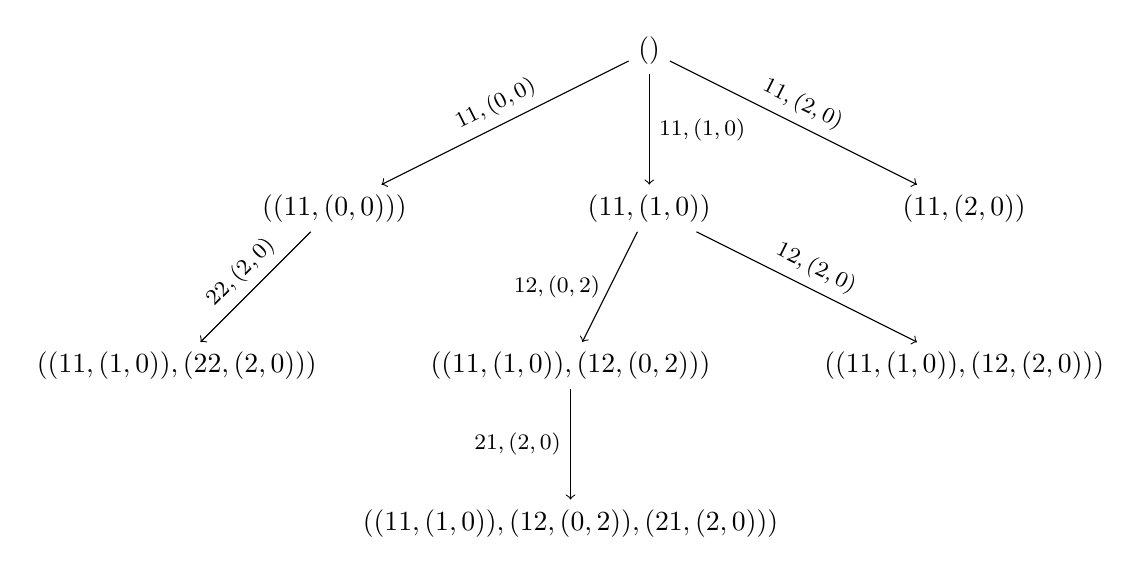
\begin{tikzpicture}
    \node (1) at (0,0) {$()$};
    \node (2) at (-4,-2) {$((11,(0,0)))$};
    \draw[->] (1) -- (2) node[pos=0.5, above, sloped] {\footnotesize{$11,(0,0)$}};
    \node (3) at (0,-2) {$(11,(1,0))$};
    \draw[->] (1) -- (3) node[pos=0.5, right] {\footnotesize{$11,(1,0)$}};
    \node (4) at (4,-2) {$(11,(2,0))$};
    \draw[->] (1) -- (4) node[pos=0.5, above, sloped] {\footnotesize{$11,(2,0)$}};
    \node (5) at (-1,-4) {$((11,(1,0)), (12,(0,2)))$};
    \draw[->] (3) -- (5) node[pos=0.5, left] {\footnotesize{$12,(0,2)$}};
    \node (6) at (4,-4) {$((11,(1,0)), (12,(2,0)))$};
    \draw[->] (3) -- (6) node[pos=0.5, above, sloped] {\footnotesize{$12,(2,0)$}};
    \node (7) at (-6,-4) {$((11,(1,0)), (22,(2,0)))$};
    \draw[->] (2) -- (7) node[pos=0.5, above,sloped] {\footnotesize{$22,(2,0)$}};
    \node (8) at (-1,-6) {$((11,(1,0)), (12,(0,2)), (21,(2,0)))$};
    \draw[->] (5) -- (8) node[pos=0.5, left] {\footnotesize{$21,(2,0)$}};
    \end{tikzpicture}
    \caption{Strom algoritmu pro [2,2]-Mastermind}
\label{fig22minmax}
\end{figure}



